\documentclass{beamer}
\usepackage{amsmath}
\usepackage[english]{babel} %set language; note: after changing this, you need to delete all auxiliary files to recompile
\usepackage[utf8]{inputenc} %define file encoding; latin1 is the other often used option
\usepackage{csquotes} % provides context sensitive quotation facilities
\usepackage{graphicx} %allows for inserting figures
\usepackage{booktabs} % for table formatting without vertical lines
\usepackage{textcomp} % allow for example using the Euro sign with \texteuro
\usepackage{stackengine}
\usepackage{wasysym}
\usepackage{tikzsymbols}
\usepackage{textcomp}
% ELIMINAR COMANDOS DE NAVEGACION%%%%%%%%%%%
\setbeamertemplate{navigation symbols}

%\newcommand{\bubblethis}[2]{
 %       \tikz[remember picture,baseline]{\node[anchor=base,inner sep=0,outer sep=0]%
 %       (#1) {\underline{#1}};\node[overlay,cloud callout,callout relative pointer={(0.2cm,-0.7cm)},%
 %       aspect=2.5,fill=yellow!90] at ($(#1.north)+(-0.5cm,1.6cm)$) {#2};}%
 %   }%
%\tikzset{face/.style={shape=circle,minimum size=4ex,shading=radial,outer sep=0pt,
 %       inner color=white!50!yellow,outer color= yellow!70!orange}}

%% Some commands to make the code easier
\newcommand{\emoticon}[1][]{%
  \node[face,#1] (emoticon) {};
  %% The eyes are fixed.
  \draw[fill=white] (-1ex,0ex) ..controls (-0.5ex,0.2ex)and(0.5ex,0.2ex)..
        (1ex,0.0ex) ..controls ( 1.5ex,1.5ex)and( 0.2ex,1.7ex)..
        (0ex,0.4ex) ..controls (-0.2ex,1.7ex)and(-1.5ex,1.5ex)..
        (-1ex,0ex)--cycle;}
\newcommand{\pupils}{
  %% standard pupils
  \fill[shift={(0.5ex,0.5ex)},rotate=80] 
       (0,0) ellipse (0.3ex and 0.15ex);
  \fill[shift={(-0.5ex,0.5ex)},rotate=100] 
       (0,0) ellipse (0.3ex and 0.15ex);}

\newcommand{\emoticonname}[1]{
  \node[below=1ex of emoticon,font=\footnotesize,
        minimum width=4cm]{#1};}
\usepackage{scalerel}
\usetikzlibrary{positioning}
\usepackage{xcolor,amssymb}
\newcommand\dangersignb[1][2ex]{%
  \scaleto{\stackengine{0.3pt}{\scalebox{1.1}[.9]{%
  \color{red}$\blacktriangle$}}{\tiny\bfseries !}{O}{c}{F}{F}{L}}{#1}%
}
\newcommand\dangersignw[1][2ex]{%
  \scaleto{\stackengine{0.3pt}{\scalebox{1.1}[.9]{%
  \color{red}$\blacktriangle$}}{\color{white}\tiny\bfseries !}{O}{c}{F}{F}{L}}{#1}%
}
\usepackage{fontawesome} % Social Icons
\usepackage{epstopdf} % allow embedding eps-figures
\usepackage{tikz} % allows drawing figures
\usepackage{amsmath,amssymb,amsthm} %advanced math facilities
\usepackage{lmodern} %uses font that support italic and bold at the same time

\usepackage{tikz}

\usepackage{tcolorbox}

\usefonttheme[onlymath]{serif} %set math font to serif ones

\definecolor{beamerblue}{rgb}{0.2,0.2,0.7} %define beamerblue color for later use

%%% defines highlight command to set text blue
\newcommand{\highlight}[1]{{\color{blue}{#1}}}


%%%%%%% commands defining backup slides so that frame numbering is correct

\newcommand{\backupbegin}{
   \newcounter{framenumberappendix}
   \setcounter{framenumberappendix}{\value{framenumber}}
}
\newcommand{\backupend}{
   \addtocounter{framenumberappendix}{-\value{framenumber}}
   \addtocounter{framenumber}{\value{framenumberappendix}}
}

\newtcolorbox{boxA}{
    fontupper = \bf,
    boxrule = 1.5pt,
    colframe = black % frame color
}

\usepackage{hyperref}

%%%% end of defining backup slides

%Specify figure caption, see also http://tex.stackexchange.com/questions/155738/caption-package-not-working-with-beamer
\setbeamertemplate{caption}{\insertcaption} %redefines caption to remove label "Figure".
%\setbeamerfont{caption}{size=\scriptsize,shape=\itshape,series=\bfseries} %sets figure  caption bold and italic and makes it smaller


\usetheme{Boadilla}

% --------------------
% Overall information
% --------------------
\title[Economía I]{Economía I \vspace{4mm}
\\ Magistral 5: Dentro de la firma}
\date{}
\author[Riottini]{Franco Riottini}
\vspace{0.4cm}
\institute[]{Universidad de San Andrés} 


\begin{document}

\begin{frame}
\titlepage
\centering

\includegraphics[scale=0.2]{../Figures/logoUDESA.jpg} 
\end{frame}

\begin{frame}
    \frametitle{El comportamiento de la firma}
    \begin{itemize}
        \item ¿Cuál es el objetivo de las empresas?
        \begin{center}
            ¡¡¡GANAR DINERO!!!
        \end{center}
        \item Seguramente los empresarios tienen otros objetivos, pero quizás los satisfacen usando parte de sus ganancias. 
        \item Las empresas que no buscan ganar dinero van a tener problemas para sobrevivir.
        \item Las decisiones que toman las empresas dependen de 
        \begin{itemize}
            \item de las características del mercado (la demanda), y
            \item de los costos de producción,
            \item ... las políticas gubernamentales (por ejemplo impuestos) van a afectar las decisiones
        \end{itemize}    
    \end{itemize}    
\end{frame}

\begin{frame}
\frametitle{Restricciones y decisiones}
\begin{itemize}
    \item La firma se enfrenta a dos grandes restricciones:
        \begin{itemize}
        \item Las características del mercado \\
        - ¿Qué es lo que los consumidores están dispuestos a comprar? \\
        - ¿Cómo se comportan las otras empresas?
        \item Sus capacidades tecnológicas \\
        - Las características de su función de producción dada por sus costos de producción
        \end{itemize}
    \item Tomando en cuenta estas restricciones, la empresa toma decisiones
    \begin{itemize}
        \item Sobre el precio al que ofrece sus productos...
        \item ... y la cantidad de este producto que va a producir
    \end{itemize}
\end{itemize} 
\end{frame}

\begin{frame}
\frametitle{¿Que información necesita la firma para decidir qué precio cobrar?}
    Para decidir qué precio cobrar, una empresa necesita información sobre la demanda
    \begin{itemize}
        \item ¿Qué es la demanda?
    La demanda es cuánto están dispuestos a pagar los consumidores potenciales por su producto
    \end{itemize}
\end{frame}

\begin{frame}
\frametitle{El problema de la firma}
\begin{itemize}
    \item Una vez que conocemos la demanda... ¿cómo se elige cuánto producir y el precio que cobrar?
    \vspace{2mm}
    \item El problema principal de la empresa es el de la maximización del beneficio
    \begin{itemize}
        \item ¿Qué es el beneficio? \vspace{2mm} \\
        \begin{center} 
        Beneficio = Ingresos Totales – Costos Totales
        \end{center}
        \vspace{2mm}
        \item ¿Qué es el ingreso total? 
        \vspace{2mm} \\ 
        El valor de la producción al precio ofrecido ($p \cdot q$)
        \vspace{2mm}
        \item ¿Qué es el costo total?
        \vspace{2mm} \\ 
        Los costos por unidad, por la cantidad de unidades producidas ($c \cdot q$)
    \end{itemize} 
\end{itemize} 
\end{frame}

\begin{frame}
\frametitle{Vamos a ser maestros pizzeros}
\centering

\includegraphics[scale=0.6]{../Figures/Tema_06.12_maestrospizzeros.jpg}
\end{frame}

\begin{frame}
    \frametitle{Pensando en los costos}
    \begin{itemize}
        \item Costos explícitos
        \begin{itemize}
            \item Harina, levadura, sal, agua, etc.
            \item Alquiler del negocio (podríamos ser los dueños pero en ese caso...)
            \item Salario de los empleados 
            \item Servicios que hay que pagar (agua, luz, gas, etc.)
        \end{itemize}
        \item Costos implícitos (Costo de oportunidad)
        \begin{itemize}
            \item El costo del capital invertido (que podría ser utilizado en otra actividad económica)
            \item El salario que perdemos por la actividad alternativa
        \end{itemize}
    \end{itemize}
\end{frame}

\begin{frame}{Beneficio Económico versus Beneficio Contable}
    \begin{itemize}
        \item El beneficio contable es la diferencia entre los ingresos obtenidos y los gastos incurridos.
        \item El beneficio económico incluye los costos de oportunidad.
        \item ¿En que piensan los contadores? En el \textbf{beneficio contable}
        \item ¿En que piensan los economistas? En el \textbf{beneficio económico}
    \end{itemize}

    \begin{boxA}
        \begin{center}
            El beneficio contable es la diferencia entre los ingresos obtenidos y los gastos incurridos mientras que el beneficio económico incluye los costos de oportunidad.
        \end{center}
    \end{boxA}
\end{frame}

\begin{frame}
    \frametitle{Alta ganancia contable, baja ganancia económica}
    \centering
    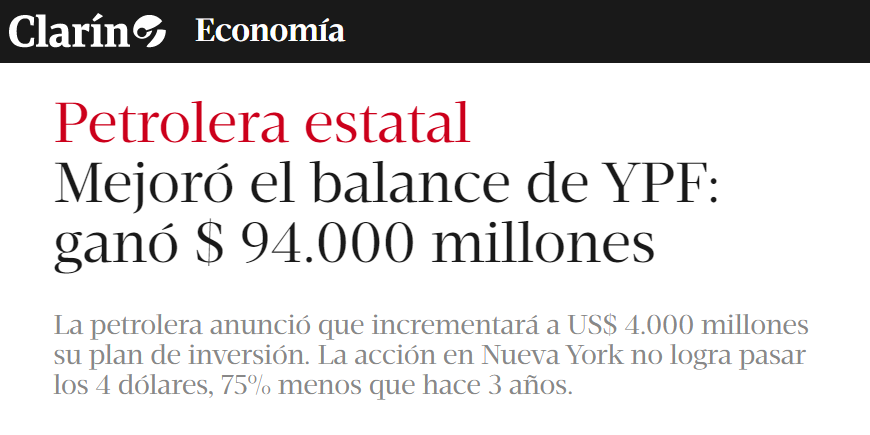
\includegraphics[scale=0.6]{../YPF.png}
\end{frame}

\begin{frame}{Regla de decisión básica}

    \begin{itemize}
        \item La regla de decisión básica es que la empresa va a producir hasta el punto en el que el beneficio económico marginal sea cero.
        \item ¿Qué es el beneficio económico marginal?
        \item ¿Qué es el ingreso marginal?
        \item ¿Qué es el costo marginal?
        \item ¿Que pasa si el ingreso marginal es mayor que el costo marginal? La empresa puede aumentar su beneficio produciendo más.
        \item ¿Qué pasa si el ingreso marginal es menor que el costo marginal? La empresa puede aumentar su beneficio produciendo menos.
    \end{itemize}

    \begin{boxA}
        \begin{center}
            Las empresas producen hasta el punto en el que el costo marginal se iguala al ingreso marginal, que es el punto en el que se maximiza el beneficio.
        \end{center}
    \end{boxA}
\end{frame}

\begin{frame}{La función de producción}
    \begin{boxA}
        \begin{center}
            La función de producción es una expresión matemática que indica la cantidad máxima de bienes que una empresa puede producir, dada su tecnología, a partir de la combinación una cantidad específica de insumos.
        \end{center}
    \end{boxA}
    Vamos a diferenciar entre el corto y el largo plazo:
    \begin{itemize}
        \item En el corto plazo puedo solo cambiar la cantidad de algunos insumos
        \begin{itemize}
            \item En el ejemplo clásico donde tengo Trabajo y Capital, puedo cambiar la cantidad de trabajo pero no la de capital
        \end{itemize}
        \item En el largo plazo puedo cambiar la cantidad de todos los insumos
        \begin{itemize}
            \item Ahora también podría cambiar la cantidad de capital, adquiriendo más maquinarias o alquilando nuevos lugares, entre muchos otros ejemplos
        \end{itemize}
    \end{itemize}
\end{frame}

\begin{frame}
\frametitle{La función de producción en el corto plazo...}
\centering
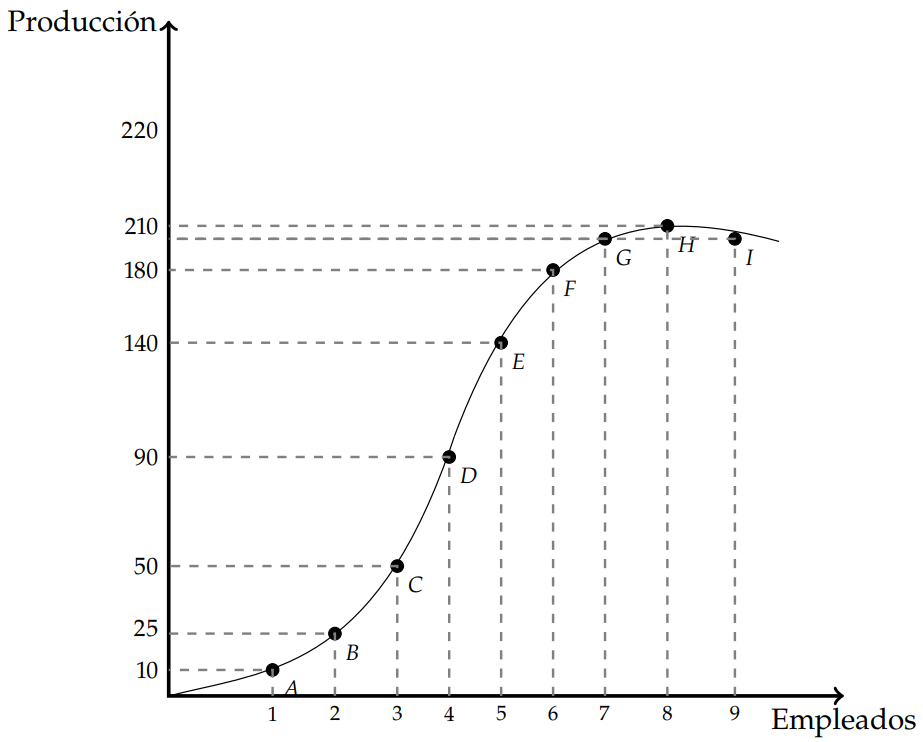
\includegraphics[scale=0.5]{../Figures/C12.1.png}
\end{frame}

\begin{frame}
    \frametitle{Contratando a un empleado adicional}
    \begin{itemize}
        \item Si observamos la función de producción anterior, la cantidad de producción que suma cada trabajador adicicional es distinta dependiendo cuantos trabajadores ya tengo
        \item Esto quiere decir que lo que cambia a medida que contrato más trabajadores es el \textbf{producto marginal}
        \item El producto marginal es la cantidad de producción adicional que se genera al aumentar la cantidad de trabajadores en una unidad
        \[ PMg = \frac{\Delta Q}{\Delta L} \]
        \item Además, esto va a cambiar el \textbf{producto medio}\dots
        \item El producto medio representa la cantidad de producto que cada trabajador genera en promedio (durante un periodo de tiempo dado)
        \[ PMe = \frac{Q}{L} \]
    \end{itemize}
\end{frame}

\begin{frame}
\frametitle{Producto marginal y medio}
\centering
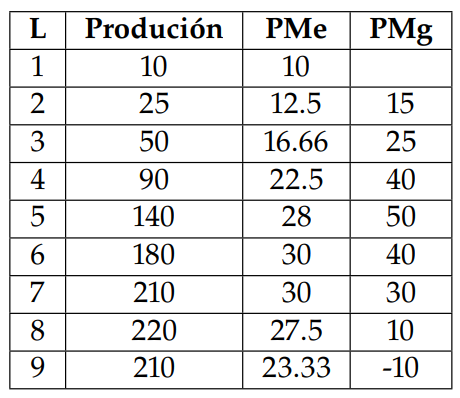
\includegraphics[scale=0.6]{../Figures/T12.3.png}
\end{frame}

\begin{frame}
    \frametitle{Producto marginal y medio}
    \centering
    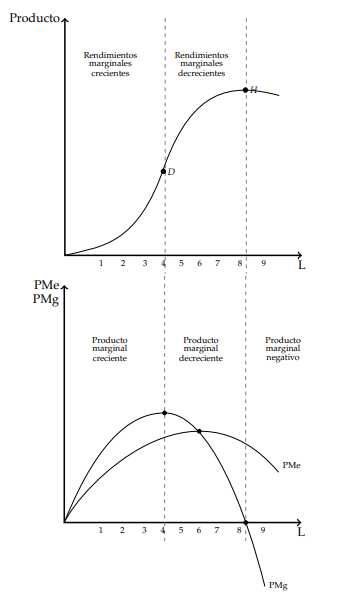
\includegraphics[scale=0.65]{../Figures/C12.7.png}
\end{frame}

\begin{frame}{Producción y costos}
\begin{itemize}
    \item La función de producción puede verse también como una función de costos
    \item ¿Por qué? Porque los costos de producción están intrinsecamente relacionados con la cantidad de producción
    \item Por ende, el producto marginal va a estar muy relacionado con el costo marginal
    \item Los costos son de dos tipos
    \begin{itemize} 
        \item Los costos fijos (no cambian con la producción)
        \item Los costos variables (cambian con la producción)
    \end{itemize}
    \item En largo plazo, vamos a asumir que todos los costos cambian con el nivel de producción\dots
    \item Si esto pasa, no hay costos fijos en el largo plazo!
\end{itemize}
\end{frame}

\begin{frame}
\frametitle{Veamos los costos fijos...}
\centering
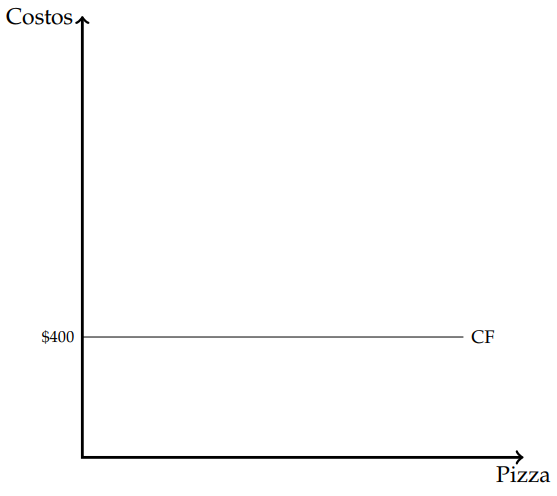
\includegraphics[scale=0.6]{../Figures/C13.1.png}
\end{frame}

\begin{frame}
\frametitle{y ahora los costos variables}
\centering
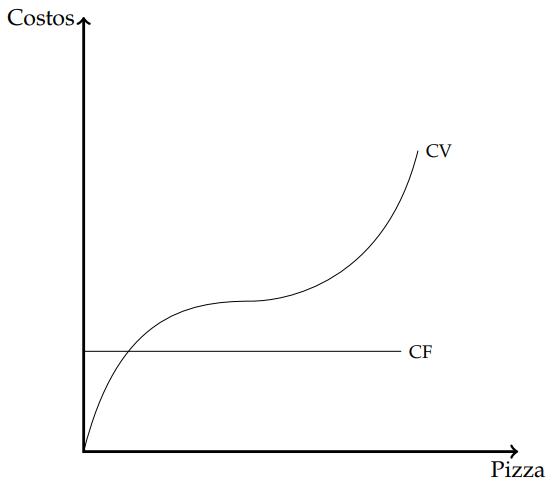
\includegraphics[scale=0.6]{../Figures/C13.2.png}
\end{frame}

\begin{frame}
    \frametitle{La forma de los costos variables}
    \centering
    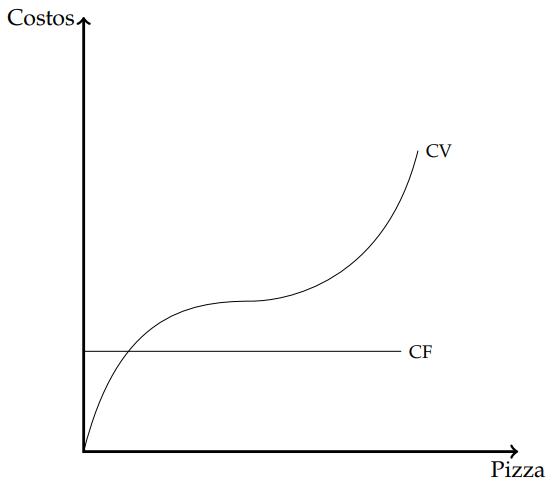
\includegraphics[scale=0.6]{../Figures/C13.2.png}
\end{frame}

\begin{frame}
\frametitle{Los costos totales}
\centering
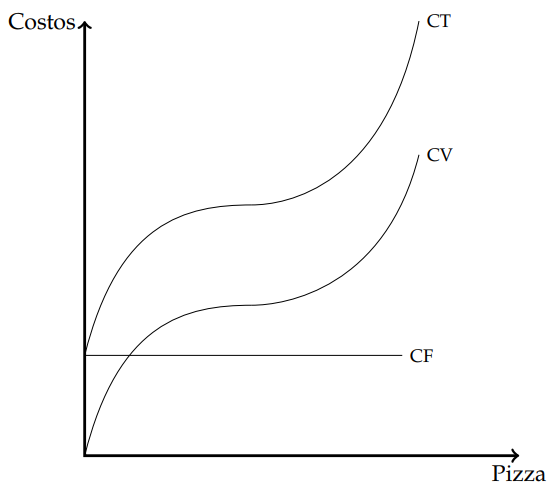
\includegraphics[scale=0.6]{../Figures/C13.3.png}
\end{frame}

\begin{frame}
\frametitle{Los costos de hacer pizzas}
\begin{itemize}
    \item Se observan dos tipos de costos: 
        \begin{itemize}
        \item Los costos fijos
        \item Los costos variables
        \end{itemize}
    \vspace{2mm}
    \item Para evaluar la cantidad de pizzas que queremos producir nos vamos a hacer dos preguntas:
        \begin{itemize}
        \item ¿Cuánto cuesta en promedio una pizza? (Costo medio)
        \item ¿Cuánto cuesta hacer una pizza adicional? (Costo marginal)
        \end{itemize}
\end{itemize}
\end{frame}

\begin{frame}
\frametitle{Costos: ¡para completar! }
\centering
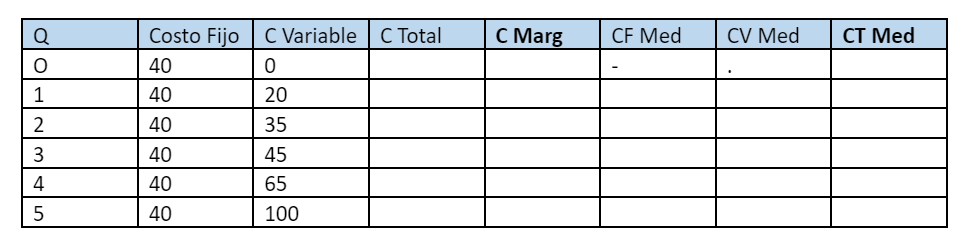
\includegraphics[scale=0.6]{../Figures/Cost1.png}
\end{frame}

\begin{frame}
\frametitle{Los costos medios y marginales}
\begin{itemize}
    \item El costo medio es el costo promedio por unidad producida
    \begin{itemize}
        \item Gráficamente es la pendiente del rayo que sale desde el origen a un punto dado de la función de costo \\
        - En el ejemplo, disminuye al principio pero luego aumentan 
    \end{itemize}
    \item El costo marginal mide el efecto sobre el costo total al producir una unidad adicional
    \begin{itemize}
        \item Gráficamente, es la pendiente de la función de costo en un punto dado \\
        - En el ejemplo, los costos marginales aumentan a medida que aumenta la producción
    \end{itemize}
\end{itemize}
\end{frame}

\begin{frame}
\frametitle{¿Cómo construir los costos medios?}
\centering
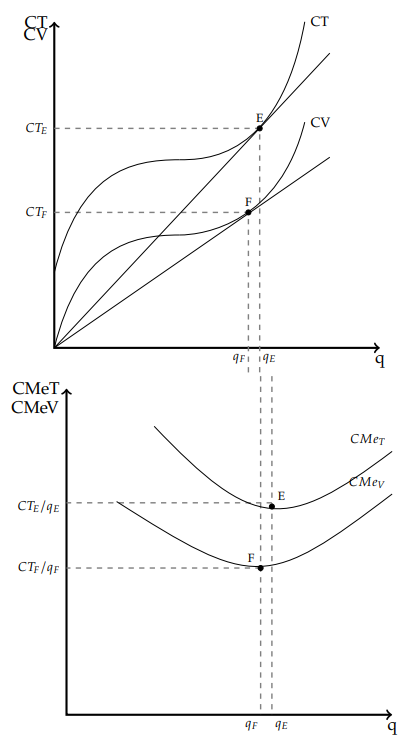
\includegraphics[scale=0.5]{../Figures/C13.6.png}
\end{frame}


\begin{frame}
\frametitle{¿Cómo construir el costo marginal?}
\centering
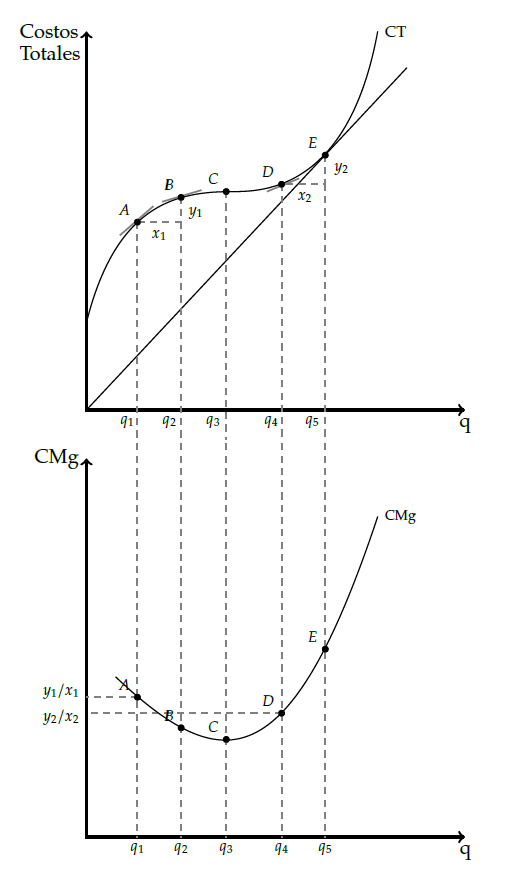
\includegraphics[scale=0.9]{../Figures/Contruyendocmg.png}
\end{frame}

\begin{frame}
\frametitle{Graficando costo medio y marginal en el mismo gráfico}
\centering
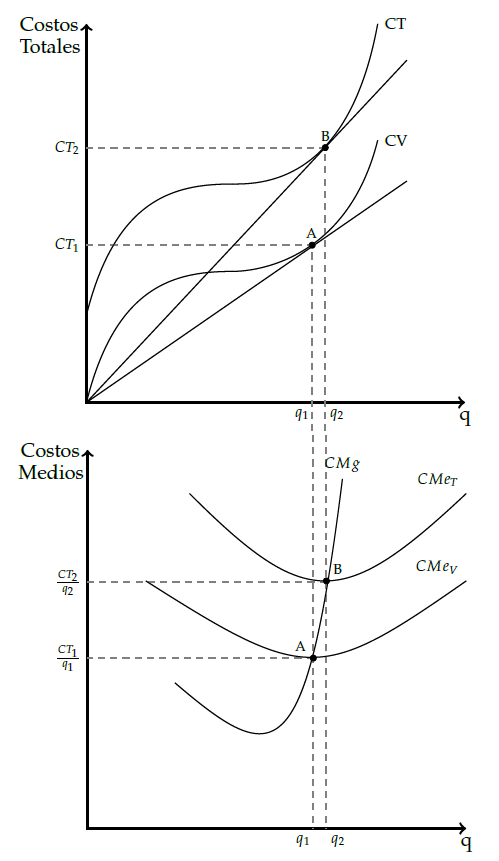
\includegraphics[scale=0.9]{../Figures/Costoscp.png}
\end{frame}

\begin{frame}
\frametitle{Las propiedades de las curvas}
\begin{itemize}
    \item El costo marginal eventualmente aumenta debido a los rendimientos marginales decrecientes.
    \item La curva de costo total promedio suele tener forma de U. Bajan los costos fijos medios y aumentan los costos variables medios.
    \item La curva de costo marginal corta la curva de costo total promedio en su nivel mínimo.
    \item Si el costo marginal es menor al costo medio, el costo medio disminuye al aumentarla producción
\end{itemize}
\end{frame}


\end{document}


